\documentclass[11pt]{beamer}
\usetheme{Madrid}
\usepackage[utf8]{inputenc}
\usepackage[german]{babel}
\usepackage[T1]{fontenc}
\usepackage{amsmath}
\usepackage{amsfonts}
\usepackage{amssymb}
\usepackage{graphicx}
\usepackage{multicol}
\usepackage{listings}
\usepackage{enumitem}
\usepackage{hyperref}
\usepackage[square,sort,comma,numbers]{natbib}
\usepackage{style/csharp}
\usepackage{minted}
\author{Florian Gehring}
\title{Vergleich zu C\#}
\subtitle{Entwicklung der Programmiersprache Java}
%\setbeamercovered{transparent} 
%\setbeamertemplate{navigation symbols}{} 
%\logo{} 
%\institute{} 
\date{18.06.2020} 
%\subject{} 

\setlist{parsep=3em}
\setlist{label=\textbullet}

\definecolor{java}{rgb}{1, 0.94, 0.8}

\newmintedfile[csharpcode]{csharp}{
bgcolor=lightgray,
linenos=true,
numberblanklines=true,
numbersep=3pt,
autogobble=true,
frame=leftline,
framerule=0.pt,
framesep=1mm,
funcnamehighlighting=true,
tabsize=4,
obeytabs=false,
mathescape=false
samepage=false, %with this setting you can force the list to appear on the same page
showspaces=false,
showtabs =false,
texcl=false,
fontsize=\small
}



\newmintedfile[javacode]{java}{
bgcolor=java,
linenos=true,
numberblanklines=true,
numbersep=3pt,
autogobble=true,
frame=leftline,
framerule=0.pt,
framesep=1mm,
funcnamehighlighting=true,
tabsize=4,
obeytabs=false,
mathescape=false
samepage=false, %with this setting you can force the list to appear on the same page
showspaces=false,
showtabs =false,
texcl=false,
fontsize=\small
}


\begin{document}
\setminted{linenos}

\begin{frame}
	\titlepage
	\begin{center}
		Dozent: Prof. Plümicke\medskip \\
		\tiny{\url{https://github.com/flo-gehring/seminar-2020-entwicklung-java/} }

	\end{center}
\end{frame}

%\begin{frame}
%\tableofcontents
%\end{frame}

% Hello World Frame
\begin{frame}{Hello, World!}
	\csharpcode{Beispielcode/scraps/hello_world.cs}
\end{frame}


\begin{frame}{Entwicklungsgeschichte}
	\begin{itemize}
		\item Entwicklung seit 2000 von Microsoft
		\item C\#-Version History von Microsoft:\cite{csharp_history}
		\begin{itemize}
					\item \glqq When you go back and look, C\# version 1.0, released with Visual Studio .NET 2002, looked a lot like Java.\grqq{}
		 \item \glqq C\# version 1.0 was a viable alternative to Java on the Windows platform.\grqq{}
		 \item \glqq And yet, C\# continued to play a bit of catch-up with Java. Java had already released versions that included generics and iterators.\grqq{} (Version 2.0)
		 \item \glqq With version 3.0, C\# had moved the language firmly out from the shadow of Java and into prominence.\grqq{} (Ende 2007)
		\end{itemize}
	\end{itemize}
\end{frame}

\begin{frame}{Ausführung}

	\begin{itemize}
		\item Virtuelle Maschine, wird zu Zwischencode kompiliert
		\item Spezifiziert durch  Common Language Infrastructure Standard
		\begin{itemize}
			\item Implementierung durch .NET, .NET Core und Mono 
			\item[$\rightarrow$] CLR (Common Language Runtime)
		\end{itemize}
	\end{itemize}
	
	\setlength{\columnseprule}{0.4pt}
	\begin{multicols}{2}
		Java \\
		\begin{itemize}
			\item Java Virtual Machine (JVM)
			\item Bytecode
		\end{itemize}

		\columnbreak

		C\#\\
		\begin{itemize}
			\item Common Language Runtime (CLR)
			\item Common Intermediate Language (CIL)
		\end{itemize}
	\end{multicols}
\end{frame}


\begin{frame}{Typsystem Allgemein}
	\begin{figure}
	\centering
		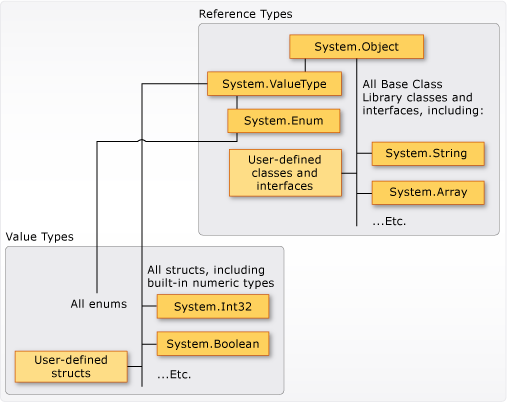
\includegraphics[width=0.7\textwidth]{bilder/value-reference-types-common-type-system.png}
		\caption{Common Type Systems (CTS) \cite{progrguide}}
	\end{figure}
\end{frame}

\begin{frame}{Werttypen}
\csharpcode[firstline=6, lastline=15, fontsize=\footnotesize]{Beispielcode/csharp/typesystem.cs}System.Int32 \\ %\lstinputlisting[linerange={6-20}]{Beispielcode/typesystem.cs}
System.Int32 -> System.ValueType -> System.Object ->
\end{frame}


\begin{frame}{Werttypen - Vergleich Java}
	\begin{itemize}
		\item In Java: Integer $\neq$ int
		\item Oft automatische Konvertierung, aber int ist kein Objekt
	\end{itemize}
	\javacode[firstline=8, lastline=14]{Beispielcode/java/test/test.java}
	
\end{frame}

\begin{frame}{Klassen}

	\begin{itemize}
		\item  Enthalten: \textbf{\texttt{properties}}, \texttt{indexers}, \texttt{events}, \texttt{operators}

		\item In C\# kann nur von einer Elternklasse geerbt werden
		\begin{itemize}
			\item Composition vs. Inheritance
		\end{itemize}
		\item Virtuelle Methoden bei Vererbung 
		\begin{itemize}
			\item Java
			\begin{itemize}
				\item (Fast) Alle Methoden sind virtuell
				\item Override wird mit \texttt{final} verhindert.
				\item \texttt{@Override} Dekorator
			\end{itemize}
			\item C\#
			\begin{itemize}
				\item Nicht alle Methoden virtuell
				\item Können mit \texttt{virtual} Modifier virtuell werden
				\item \texttt{new} und \texttt{override} Keyword 
			\end{itemize}
		\end{itemize}
	\end{itemize}
\end{frame}


%---------------------
% 		Generics		-
%---------------------

\begin{frame}{Generics - C\#}
	\csharpcode[firstline=2,lastline=14]{Beispielcode/scraps/generics-1.cs}
\end{frame}

\begin{frame}{Generics - Java}
	\javacode{Beispielcode/java/GenericDemo.java}
\end{frame}

\begin{frame}{Generics - Subtyping}
	\javacode{Beispielcode/java/Box.java}
	\javacode[firstline=6, lastline=9]{Beispielcode/java/BoxDemo.java}
\end{frame}

\begin{frame}{Generics - Subtyping}
	\begin{figure}
			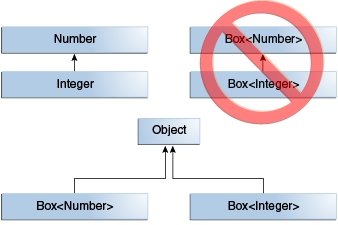
\includegraphics[width=0.66\textwidth]{bilder/generics-subtypeRelationship.png}
			\caption{Subtype Relationship \cite{java_generics_inheritance}}
	\end{figure}
\end{frame}

\begin{frame}{Covarianz und Contravarianz}
	\begin{itemize}
		\item \glqq Covariance and contravariance are terms that refer to the ability to use a more derived type (more specific) or a less derived type (less specific) than originally specified.\grqq{} \cite{csharp_docs_variance}
		\item Covariante Typparameter  sehen wie \glqq gewöhnlicher\grqq{} Polymorphismus aus.
		\csharpcode[firstline=23, lastline=24]{Beispielcode/scraps/generics-1.cs}
		\item Contravarianz:
		\csharpcode[firstline=28, lastline=29]{Beispielcode/scraps/generics-1.cs}
	\end{itemize}

		%\csharpcode[firstline=21, lastline=22]{Beispielcode/scraps/generics-1.cs}
\end{frame}

\begin{frame}{Contravarianz (1)}
\tiny{
\texttt{Circle} implementiert \texttt{Shape}. \texttt{IComparer<T>} ist als Contravariant markiert.}
\csharpcode[fontsize=\tiny, lastline=24]{Beispielcode/csharp/ContravariantDemo.cs}
Beispiel von \cite{csharp_example_contravariance}
\end{frame}

\begin{frame}{Contravarianz (2)}
\tiny{
\texttt{Circle} implementiert \texttt{Shape}. \texttt{IComparer<T>} ist als Contravariant markiert.}
\csharpcode[fontsize=\tiny, firstline=17, lastline=39]{Beispielcode/csharp/ContravariantDemo.cs}
Beispiel von \cite{csharp_example_contravariance}
\end{frame}


\begin{frame}{C\# - Variante Interfaces}
	\csharpcode[fontsize=\tiny]{Beispielcode/csharp/variant_interfaces.cs}
\end{frame}


\begin{frame}{C\# - Invariante Klassen}
	Erinnerung: 
	\csharpcode[firstline=4, lastline=4]{Beispielcode/csharp/variant_interfaces.cs}
	Variablen die eine Klasse als Typ haben sind invariant:
	\csharpcode[firstline=5, lastline=12]{Beispielcode/csharp/invariant_classes.cs}
\end{frame}

\begin{frame}{Varianz in Java: Wildcards}
		Wildcards mit upper (\texttt{extends}) oder lower (\texttt{super}) Bound. \texttt{extends} gilt auch für implementierte Interfaces.
		\javacode[firstline=11, lastline=12]{Beispielcode/java/BoxDemo.java}
		Anwendungsbeispiel:
		\javacode[firstline=15, lastline=21]{Beispielcode/java/BoxDemo.java}
\end{frame}

\begin{frame}{Wildcards}

		\javacode[fontsize=\tiny, firstline=53, lastline=55]{Beispielcode/java/test/GenericTest.java}
		Contravariant (\glqq in\grqq{}) Write-Only
				\javacode[fontsize=\tiny, firstline=57, lastline=63]{Beispielcode/java/test/GenericTest.java}
	Covariant (\glqq out\grqq{}) Read-Only
		\javacode[fontsize=\tiny, firstline=65, lastline=71]{Beispielcode/java/test/GenericTest.java}

\end{frame}


\begin{frame}{Java Konzept: Type Erasure}
	\begin{itemize}
	\item Java unterstützt auf Bytecode Ebene keine Generics
	\begin{enumerate}
		\item Keine generischen Typinformationen zur Laufzeit
	\end{enumerate}
	\item Generisches Argument wird durch möglichst spezifischen Typ ersetzt
	\end{itemize}
	\javacode{Beispielcode/scraps/type_erasure.java}
\end{frame}




%-------------------------------------
% 		Type Erasure Konsequenzen 	-
%-------------------------------------

\begin{frame}{Type Erasure: Methoden}
	\begin{figure}
		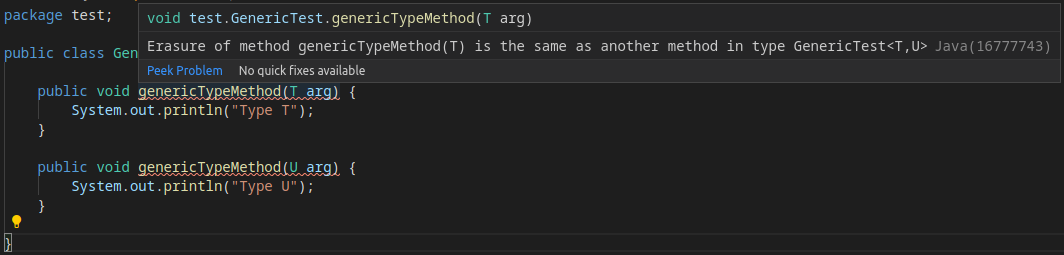
\includegraphics[width=\textwidth]{bilder/java_type_erasure.png}
	\end{figure}
	\csharpcode[firstline=2, lastline=8]{Beispielcode/csharp/GenericSort.cs}
\end{frame}

\begin{frame}{Type Erasure: Typen Generischer Klassen}
	Java
	\javacode[firstline=12, lastline=18]{Beispielcode/java/test/GenericTest.java}
	$C\#$
	\csharpcode[firstline=10, lastline=14]{Beispielcode/csharp/GenericSort.cs}
\end{frame}

\begin{frame}{Type Erasure: Objekt Instanziierung}
	Java
	\javacode[firstline=27, lastline=35]{Beispielcode/java/test/GenericTest.java}
	$C\#$
	\csharpcode[firstline=20, lastline=22]{Beispielcode/csharp/GenericSort.cs}
\end{frame}

\begin{frame}{Type Erasure: Statische Methoden}
	\begin{figure}
		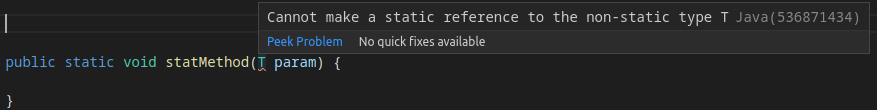
\includegraphics[width=\textwidth]{bilder/java_no_static_methods.png}
	\end{figure}
	
	$C\#$
	\csharpcode[firstline=25, lastline=40,fontsize=\tiny]{Beispielcode/csharp/GenericSort.cs}
\end{frame}

\begin{frame}{Generics - Reflection}
\begin{itemize}
	\item Java 
	\begin{itemize}
		\item Es ist trotz Type Erasure teilweise möglich mithilfe von \texttt{java.lang.reflection} während der Laufzeit auf die Parametrisierten Typen zuzugreifen. 
		\item \glqq Umweg\grqq{} über Superclass
		\item Andere Möglichkeit: Bei Konstruktion immer Klasse mit übergeben.
	\end{itemize}
	\item C\# 
	\begin{itemize}
		\item Besserer Unterstützung für generische Reflektion
	\end{itemize}
\end{itemize}
\end{frame}

%-------------------------
% 		Delegates		-
%-------------------------

% Delegates
\begin{frame}{Delegates}
\begin{itemize}
 	\item \texttt{Delegate} sind Referenz\textbf{typen} (Objekte)
 	\item Sie kapseln die Funktionalität einer (anonymen) Methode
 	\item Die Methode wird mittels des Delegats aufgerufen
\end{itemize}
\csharpcode[firstline=3, lastline=4]{Beispielcode/csharp/delegates.cs}
	
\end{frame}
\begin{frame}{Delegate}
	Erstes Beispiel:
	\csharpcode[firstline=4, lastline=18]{Beispielcode/csharp/delegates.cs}
\end{frame}

\begin{frame}{Delegate}
	Initialisierung Möglich als: Methode mit Namen, Anonyme Methode und Lambda Funktion
	\csharpcode[firstline=35, lastline=41]{Beispielcode/csharp/delegates.cs}
\end{frame}

\begin{frame}{Delegates - Invocation List}
	\begin{itemize}
		\item  Eine Kombination von Delegaten ist möglich
		\item Methoden \texttt{TimesTwo (d1)} und \texttt{TimesThree} werden nacheinander mit 2 aufgerufen
		\begin{itemize}
			\item Delegatenaufruf gibt jetzt \texttt{void} zurück
		\end{itemize}
	\end{itemize}
	\csharpcode[firstline=27, lastline=30]{Beispielcode/csharp/delegates.cs}
\end{frame}

\begin{frame}{Java - Functional Interfaces}
	\javacode{Beispielcode/java/DelegMult.java}
	\javacode[firstline=3, lastline=12]{Beispielcode/java/UseFunction.java}

\end{frame}

\begin{frame}{Generische Delegate und Varianz}
	\begin{itemize}
	 	\item Ein Delegat-Typ akzeptiert auch Delegate mit:
	 	\begin{itemize}
	 		\item \glqq More Derived Types\grqq{} als Rückgabewert (Covarianz)
	 		\item \glqq Less Derived Types\grqq{} als Parameter (Contravarianz)
	 		\item Implizite Konvertierung, falls \texttt{in} bzw. \texttt{out} Keyword vorhanden
	 	\end{itemize}
	\end{itemize}
	\csharpcode[fontsize=\tiny]{Beispielcode/csharp/GenericDelegates.cs}
\end{frame}

\begin{frame}{Functional Interfaces und Varianz}
	Co- und Contravarianz in Functional Interfaces lässt sich ebenfalls über Wildcards realisieren.
	\javacode[fontsize=\tiny]{Beispielcode/java/GenericFunctionalInterfaces.java}
\end{frame}

\begin{frame}{Delegate - Vergleich Java}
	\begin{itemize}
		\item Java: Functional Interfaces
		\begin{itemize}
			\item bestehend aus einer Funktion
			\item Automatisches Casten von Lambda-Ausdrücken
			\item \glqq Lambda expressions let you express instances of single-method classes more compactly.\grqq
			\item \texttt{@FunctionalInterface} Annotation		
		\end{itemize}
		\item Man sieht nicht am Datentyp, dass es sich um eine Funktion handelt
		\item Vgl. Vortrag letztes Mal: \glqq Real Function Types\grqq
	\end{itemize}
\end{frame}

%-------------------------
% 		Quellen	    		-
%-------------------------

\begin{frame}{Quellen}
\begin{thebibliography}{99}
\fontsize{6pt}{7.2}\selectfont
	\bibitem{progrguide}"Programming Guide C\#", \url{https://docs.microsoft.com/de-de/dotnet/csharp/programming-guide/}, 05.06.2020
	\bibitem{spec_csharp} C\# Language Specification, \url{https://docs.microsoft.com/de-de/dotnet/csharp/language-reference/language-specification/introduction}, 05.06.2020
   \bibitem{intro_csharp}Introduction to C\#, \url{https://docs.microsoft.com/de-de/dotnet/csharp/language-reference/language-specification/introduction}, 06.06.2020

 \bibitem{so_var_java}'"What is the equivalent of the C\# 'var' keyword in Java?"', 
 \url{https://stackoverflow.com/a/49598148}, 05.06.2020
 \bibitem{interview_virtual}'Interview with C\# Designer', \url{https://www.artima.com/intv/nonvirtual.html}, 06.06.2020
 \bibitem{java_generics} 'Java Generics' \url{https://docs.oracle.com/javase/tutorial/java/generics/restrictions.html}, 08.06.2020
 \bibitem{blog_vgl_generics} 'Blogpost C\# / Java Generics', \url{http://www.jprl.com/Blog/archive/development/2007/Aug-31.html}, 09.06.2020
 \bibitem{java_reflection_get_types} 'SO: Get Actual Types', \url{https://stackoverflow.com/a/5684761}, 09.06.2020
 \bibitem{java_generics_inheritance} 'Java Generics: Inheritance', \url{https://docs.oracle.com/javase/tutorial/java/generics/inheritance.html}
 \bibitem{csharp_docs_variance} 'Covariance and Contravariance', \url{https://docs.microsoft.com/en-us/dotnet/standard/generics/covariance-and-contravariance}, 13.06.2020
 \bibitem{csharp_example_contravariance} 'Beispiel Contravariance', \url{https://docs.microsoft.com/en-us/dotnet/standard/generics/covariance-and-contravariance}, 13.06.2020
\bibitem{csharp_history} 'C\# Geschichte', \url{https://docs.microsoft.com/en-us/dotnet/csharp/whats-new/csharp-version-history}, 15.06.2020
\end{thebibliography}
\end{frame}
\end{document}
